\section{Spielregeln und Benutzerinteraktion}
Damit die Benutzerinteraktion funktioniert, müssen zunächst die Spielregeln ins Spiel eingebunden werden. Das Spiel das 8er- Ball-Billiard: \\
 8er Ball wird mit einem Spielball (weiss) und 15 nummerierten farbigen Kugeln gespielt. 14 der farbigen Kugeln werden in zwei Gruppen eingeteilt. Nr. 1 bis 7 sind vollfarbige (volle) Kugeln. Nr.9 bis 15 sind gestreiftfarbige (halbe) Kugeln. Zu Beginn werden alle 15 farbigen Bälle mit dem Dreieck so aufgestellt, dass die vorderste Kugel des Dreiecks auf dem Fusspunkt zu liegen kommt. Ziel des Spieles ist es, zuerst eine Serie von vollen oder halben Bällen und zuletzt den 8er Ball in die Löchern zu versenken. Jeweils der Gewinner eines Spieles eröffnet das nächste Spiel( Alternativ kann auch abwechslungsweise angespielt werden).

\subsection{Spielregeln}
Sobald der erste Spieler seinen Zug gemacht hat, started das Spiel.
Sollte der Spieler einen Ball eingelocht haben, überprüft die Spiellogik, ob es sich hierbei um eine vollen Ball handelt oder halben Ball. Entsprechend wird dabei der Balltyp des Spielers auf 'True' für einen vollen Ball oder auf 'False' für einen halben Ball gesetzt. Anschließend darf der derzeitig aktuelle Spieler einen weiteren Zug machen. \begin{equation}
BallTyp = \begin{cases}
True, & \text{ Für Volle Kugel } \\
False, & \text{ Für Halbe Kugel }
\end{cases}
\end{equation}

\begin{equation}
currentPlayer = \begin{cases}
0, & \text{ Für Ersten Spieler } \\
1, & \text{ Für Zweiten Spieler }
\end{cases}
\end{equation}

Hat der Spieler den Ball nicht eingelocht, dann wird der Spieler gewechselt.

dabei wird der BallType beim ersten spielzug nicht gesetzt, da niemand eine Farbe zugeordnet bekommen hat.
Um das Spiel zu Gewinnen muss man alle Kugeln eingelocht haben, die für den Spieler zugewiesen wurden. Die Letzte Kugel ist die Schwarze Kugel. Sollte diese versenkt worden sein, bevor alle Kugeln des Spielers versenkt sind, dann hat der Aktuelle Spieler entsprechen Verloren und ein Pop-up Fenster erscheint. Andernfalls hat Er  Gewonnen.

\subsection{Benutzerinteraktion}

Bevor ein Benutzer das Programm gestartet hat, müssen vorher einige voraussetzungen erfüllt werden. Das Programm benötigt zu ausführung eine Kamera. Diese wird zum Kalibrieren des Spielfeldes benötigt. Sollte die Kamera verbunden worden sein, so muss sie nun auf das Programm-Fenster zeigen. Zu Begin bei der Ausführung des Programms, wird ein Pop-up Fenster angezeigt, welche fragt ob die Kalibrierung gestartet werden kann(siehe Abbildung 3.6: Kalibrierung-Pop-up).
 \begin{figure}[h]
	\centering
	\caption{Kalibrierung-Pop-up}
	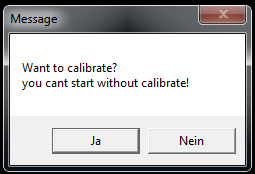
\includegraphics[width=\textwidth/3]{bilder/Calibrate-Popup.png}
\end{figure}\\
Mit dem Drücken des 'Ja'-Knopfes wird ein Signal richtung der Kamerakalibrierung geschickt und sie wird gestartet. Sollte 'Nein' gedrückt worden sein, so wird das Programm geschlosse, da das Programm die kalibrierung benötigt.
Nach der Kalibrierung wird ein weiteres Pop-up Fenster angezeigt, ob man das Spiel nun starten möchte. Wenn 'Ja' gedrückt wird, dann wird das ganze Spielfeld angezeigt. 
 \begin{figure}[h]
	\centering
	\caption{StartGame-Pop-up}
	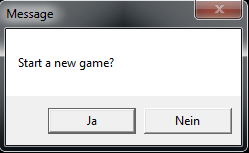
\includegraphics[width=\textwidth/3]{bilder/startGame-Popup.png}
\end{figure}\\
Nebenbei werden auch die Labels für den CurrentPlayer sowie des Balltypen angezeigt.
Das Spiel kann nun gespielt werden mit einem Queue. Hierbei muss man mit dem  Queue versuchen die weiße Kugel anzustoßen. Wichtig dabei ist, das die Kamera eingeschaltet bleiben muss.
\\\\\\
Als zusätliche funktion, hat der Spieler die möglichkeit mit der maus zu spielen(siehe Abb. 3.7: Maus Funktion), indem er sie entprechend zu der weißen kugel schlägt.
\begin{figure}[h]
	\centering
	\caption{Maus Funktion}
	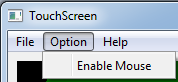
\includegraphics[width=\textwidth/3]{bilder/option-MenuBar.png}
\end{figure}\\\\
Unter File(siehe Abbildung 3.8: Start New Game) hat der Benutzer die möglichkeit das Spiel zurück zu setzten bzw. ein neues Spiel zu starten.
\begin{figure}[h]
	\centering
	\caption{Start New Game}
	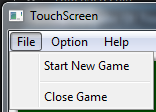
\includegraphics[width=\textwidth/3]{bilder/File-MenuBar.png}
\end{figure}\\

